\chapter{Predikaatlogica}\label{ch:predicaten}
In hoofdstuk \ref{ch:proposities} hebben we de propositielogica ge\"introduceerd als een formalisme waarmee redeneringen kunnen worden beschreven. Hierbij konden redeneringen worden geanalyseerd tot op het niveau van enkelvoudige beweringen. Een groot aantal redeneringen, ook wiskundige, kan niet met behulp van de propositielogica worden geanalyseerd. Immers, de interne structuur van de enkelvoudige beweringen wordt buiten beschouwing gelaten. Als eerste voorbeeld komen we terug op de postbode uit het eerste hoofdstuk.

De redenering begon als volgt: Stel dat de bewering `er is een adres waarop vier of meer stukken zijn afgeleverd' niet waar is, dan geldt: `voor alle adressen zijn er hoogstens drie stukken afgeleverd'. Voor het redeneren met \textit{vier of meer} en \textit{hoogstens drie} kunnen we nog wel af met gewone rekenregels, maar voor het redeneren met \textit{er is een} en \textit{voor alle} hebben we nog niets.

De taal van de propositielogica is voor veel toepassingen te arm. Dat bleek al in de Klassieke Oudheid, waar logici allerlei redeneerpatronen vonden die te maken hebben met de manier waarop wij in natuurlijke taal objecten beschrijven, en hun eigenschappen en relaties. Dan gaan andere uitdrukkingen een sleutelrol spelen dan connectieven als `niet' of `en', met name de \textit{kwantoren} `alle' en `sommige'. Maar net als in hoofdstuk \ref{ch:proposities} komt deze noodzaak tot uitbreiding het scherpst naar voren als we kijken naar wiskundig redeneren, en dus beginnen we ook weer daar om te zien wat voor rijker logisch systeem we nu nodig hebben.

In de wiskunde doen we graag algemene uitspraken over objecten uit een oneindige verzameling en van de logica verlangen we dat we deze uitspraken heel precies kunnen weergeven, en er de juiste gevolgen uit af kunnen leiden. De propositielogica is hiervoor niet altijd geschikt. Bijvoorbeeld de uitspraak:
\begin{quote}
    `elk even getal groter dan 2 is de som van twee priemgetallen' (het zogenaamde vermoeden van Goldbach)
\end{quote}
kan niet goed worden weergegeven in propositielogica.

Wat bedoelen we hier met `goed weergegeven'? Om dat te zien, doen we een klein `gedachten-experiment': stel dat we wel een geschikte formule uit de propositielogica hadden, hoe zou die er dan uit moeten zien? Aangezien er in de uitspraak geen voegwoorden te onderscheiden zijn, zouden we de uitspraak als een propositieletter moeten weergeven, zeg door `$p$'.

Beschouw nu de uitspraak:
\begin{quote}
    `2018 is de som van twee priemgetallen'
\end{quote}
Dit volgt uit het vermoeden van Goldbach, dat wil zeggen, als het vermoeden van Goldbach juist is, dan is 2018 inderdaad te schrijven als de som van twee priemgetallen. Maar `2018 is de som van twee priemgetallen' is een andere uitspraak dan het vermoeden van Goldbach. Er zit niets anders op dan hiervoor een andere propositieletter te kiezen, zeg $q$. Maar dan doet zich het probleem voor dat $p\not\vdash q$, dat wil zeggen, $q$ is geen logisch gevolg van $p$, want $p$ kan waar zijn terwijl $q$ onwaar is. Het antwoord op de vraag of $q$ een logisch gevolg is van $p$, staat namelijk los van de relatie tussen de uitspraken waar $p$ en $q$ vertalingen van zouden moeten zijn: de symbolen $p$ en $q$ zijn bij wijze van spreken `losgeweekt' van de getaltheoretische context.

De conclusie is dus dat $p$ geen goede weergave is van het vermoeden van Goldbach, en eigenlijk lag dat ook wel voor de had: de interne structuur van de uitspraak is niet in de formule $p$ terug te vinden.

Een andere poging om `Goldbach' in propositielogica weer te geven is: laat $p_i$ staan voor `$i$ is de som van twee priemgetallen'. Dan zouden we het vermoeden van Goldbach door een oneindig lange conjunctie kunnen weergeven: $p_4\wedge p_6\wedge p_8\wedge p_{10}\wedge\ldots$. Dit zou inderdaad $p_{2018}$ tot gevolg hebben. Maar een oneindig lange conjuctie is geen `formule' volgens definitie \ref{def:prop} van de taal van de propositielogica. We kunnen namelijk eenvoudig inzien dat iedere formule een eindig aantal symbolen bevat. Lange conjunctie mag, maar oneindige niet. Dus ook deze weg loopt in eerste instantie dood.

Het systeem van de predikaatlogica, waarmee we in de komende hoofdstukken kennismaken, heeft een veel grotere uitdrukkingskracht dan de propositielogica, waar ze een verfijning en uitbreiding van is. Het vermoeden van Goldbach en zijn gevolgen kunnen we in predikaatlogica w\'el goed weergeven. We maken eerst kennis met de taal van de predikaatlogica en met een methode om situaties aan te geven waarin een predikaatlogische formule waar is. In het volgende hoofdstuk kijken we naar het interpreteren van predikaatlogische formules en naar predikaatlogisch gevolg.

\section{Bouwstenen van de predikaatlogica}
In de propositielogica konden we een eenvoudige uitspraak als `Judith schaakt' alleen maar weergeven door een propositieletter. In de predikaatlogica kunnen we de interne structuur van zulke uitspraken zichtbaar maken.

\begin{example}\label{vb:pred:1}
`Judith schaakt' wordt in predikaatlogica weergegeven als $S(j)$. Hierin staat $S$ voor de eigenschap `schaken' die toekomt aan het object `Judith', dat met $j$ is aangeduid (`object' wordt hier in algemene zin gebruikt: daaronder vallen ook menselijke individuen). De eigenschap staat voorop, het object er tussen haakjes achter.
\end{example}

De predikaatlogica bevat uitdrukkingen die \textit{predikaten} (dat wil zeggen: eigenschappen van objecten en relaties tussen objecten) aangeven: dat noemen we \textit{predikaatsymbolen}. Daarnaast zien we namen voor objecten: de \textit{constanten}. In het voorbeeld is $S$ dus een predikaatsymbool en $j$ een constante. Voor predikaatsymbolen gebruiken we hoofdletters $A,\ldots,Z$ of speciale symbolen zoals `='. Voor constanten worden kleine letters $a,\ldots, t$ en ook wel getallen gebruikt. De letters $u,\ldots,z$ gebruiken we als variabelen.

We kiezen over het algemeen letters die makkelijk te onthouden zijn, bijvoorbeeld de beginletter van het met het predikaatsymbool overeenkomstige woord. Maar logisch gezien is er geen enkel verband tussen een letter en de daarmee bedoelde eigenschap (en eigenlijk is dit evenmin zo als we getallen gebruiken als constante symbolen), dus dit verband moeten we expliciet aangeven door middel van een zogeheten vertaalsleutel.

\begin{example}\label{vb:pred:2}
De uitspraken:
\begin{itemize}
    \item Marie is wiskundige.
    \item 5 is een priemgetal.
\end{itemize}
kunnen in predikaatlogica worden weergegeven door respectievelijk:
\begin{itemize}
    \item $m:$ Marie
    \item $5:$ het getal vijf
    \item $W:$ is wiskundige
    \item $P:$ is een priemgetal
\end{itemize}
In het vervolg laten we het vermelden van de vertaalsleutel vaak achterwege wanneer deze erg voor de hand ligt. De predikaatsymbolen in dit voorbeeld zijn dus $W$ en $P$ en de constanten zijn $m$ en $5$. Ook zullen we meestal zeggen dat we de constante $5$ vertalen als het getal $5$, als `zichzelf', als het ware; ook al is daar formeel een verschil tussen.
\end{example}

Ook relaties, zowel in wiskundige als in andere zin, kunnen we logisch aanduiden met predikaatsymbolen. Het volgende voorbeeld laat zien dat we dan ook weer moeiteloos van wiskundige taal op natuurlijke taal kunnen overstappen.

\begin{example}\label{vb:pred:3}
De uitspraken:
\begin{itemize}
    \item Jan houdt van Marie.
    \item 5 is groter dan 3.
\end{itemize}
kunnen in predikaatlogica worden vertaald als:
\begin{itemize}
    \item $H(j, m)$
    \item $G(5, 3)$
\end{itemize}
Merk op dat ook hier de predikaatsymbolen voorop staan, gevolgd door de objecten tussen haakjes en door komma's gescheiden. De weergave $G(5,3)$ wijkt echter wel erg af van de wiskundige praktijk. In plaats van $G$ gebruiken we dan altijd het symbool `$>$'; en dat wordt gewoon tussen de constanten in geschreven, zodat we de volgende bekende notatie gebruiken:
\begin{itemize}
    \item $5>3$
\end{itemize}
\end{example}

Ook andere gangbare relaties zoals gelijkheid `$=$', kleiner dan `$<$' en groter dan of gelijk aan `$\geq$', worden door de bekende symbolen weergeven en tussen de constanten geschreven in plaats van ervoor.

Predikaatsymbolen zoals $P$ en $W$ in voorbeeld \ref{vb:pred:2} worden door slechts \'e\'en constante gevolgd: zulke predikaatsymbolen worden \textit{\'e\'enplaatsig} genoemd. De predikaatsymbolen in voorbeeld \ref{vb:pred:3} hebben twee constanten bij zich: we noemen deze \textit{tweeplaatsig}.

Eigenschappen worden dus in de regel door 1-plaatsige predikaatsymbolen weergeven, binaire relaties door 2-plaatsige. Hier houdt het niet mee op: er zijn ook 3-plaatsige, 4-plaatsige en in het algemeen $n$-plaatsige predikaatsymbolen.

\begin{example}\label{vb:pred:4}
De uitspraken:
\begin{itemize}
    \item $1/2$ ligt tussen 0 en 1.
    \item Marie geeft Jan `De Aanslag'.
    \item punt $D$ heeft dezelfde afstand tot $P$, $Q$ en $R$.
\end{itemize}
kunnen in predikaatlogica worden weergegeven door:
\begin{itemize}
    \item $T(1/2,0,1)$
    \item $G(m,j,a)$
    \item $A(d,p,q,r)$
\end{itemize}
\end{example}

Naast constanten, die elk een bepaald vast object aanduiden, willen we ook graag over symbolen beschikken die \textit{verschillende} objecten kunnen aanduiden.
\begin{example}
De uitspraken:
\begin{itemize}
    \item $x$ is groter dan 3.
    \item Marie houdt van hem.
\end{itemize}
kunnen worden weergegeven door:
\begin{itemize}
    \item $x>3$
    \item $H(m,x)$
\end{itemize}
In beide gevallen hangt het van de situatie af wat `$x$' (of `hem') is. Bijvoorbeeld, als $x=5$, dan krijgen we $5>3$, maar als $x=10$, dan krijgen we $10>3$.
\end{example}

Net als in de wiskunde noemen we $x$ een variabele. De letters $y$ en $z$, en soms ook $u$ en $v$, worden eveneens gebruikt als variabele, eventueel vergezeld van een accent ($x'$) of een index ($x_0$). Zo'n `variabele constante' $x$ (een naamgeving waar we niet omheen kunnen, ook al lijkt het tegenstrijdig) lijkt dus wat op de propositionele formulevariabelen zoals $\varphi$ en $\psi$. Er is echter een belangrijk verschil; variabele constanten zoals $x$ gaan echt deel uitmaken van de predikaatlogische taal. Terwijl formulevariabelen niet meer dan `plaatsvervangende' formules zijn, die we later nog kunnen concretiseren om er echte formules van te maken.

In de predikaatlogica hebben we geen propositieletters. Het is wel van belang dat we beschikken over haakjes en connectieven. Met behulp van de connectieven $\neg,\wedge,\vee,\rightarrow$ en $\leftrightarrow$ kunnen we nu ook ingewikkeldere uitspraken weergeven in predikaatlogica. Dit zou je ook `vertalen' kunnen noemen.

\begin{example}
De uitspraken:
\begin{itemize}
    \item Jan houdt van Marie, maar Marie niet van Jan.
    \item $x$ is groter dan 0 of $y$ is kleiner dan 1.
    \item als $x$ groter is dan 3 en een priemgetal is, dan is $x$ oneven.
\end{itemize}
kunnen vertaald worden als:
\begin{itemize}
    \item $H(j,m)\wedge\neg H(m,j)$
    \item $x>0\vee y<1$
    \item $(x>3\wedge P(x))\rightarrow O(x)$
\end{itemize}
De laatste uitspraak gaat dus over een specifieke, zij het nog onbekende waarde voor $x$. Ze wordt ook vaak algemener opgevat, namelijk als: `\textit{voor elke $x$ geldt}, dat als $x$ groter is dan 3 en een priemgetal, dan is $x$ oneven'. Dat bedoelen we hier niet, maar dat kunnen we wel in predikaatlogica uitdrukken, en daar vervolgende we nu mee.
\end{example}

Algemene feiten van het soort `voor elke $x$ geldt dat als $x$ een priemgetal groter dan 3 is, dan is $x$ oneven' zijn heel precies uit te drukken in predikaatlogica. De formule $(x>3\wedge P(x))\rightarrow O(x)$ voldoet echter niet, want daarin heeft $x$ nog steeds een specifieke (maar een `verzwegen') waarde. Wat we expliciet moeten aangeven, is dat hier alle mogelijke waarden voor $x$ op het oog hebben. Dit doen we door de zogenaamde kwantor $\forall$ (spreek uit: `voor elke \ldots' of `voor alle \ldots') en de betreffende variabele voor de formule te zetten, resulterend in:
$$\forall x(x>3\wedge P(x))\rightarrow O(x)$$
Het symbool $\forall$ wordt (al dan niet in combinatie met variabele) de \textit{universele kwantor} of \textit{al-kwantor} genoemd.

\begin{aside}[Kwantoren (ook wel quantoren)]\mbox{}\\
Kwantificatie is een begrip uit de wiskunde en taalkunde om uitspraken te doen over meerdere elementen van een \textit{domain of discourse} (een universum waarover uitspraken worden gedaan). In de natuurlijke taal kennen we meerdere kwantoren, zoals \textit{voor alle}, \textit{voor sommige}, \textit{vele}, \textit{enige}, \textit{geen enkele}.

Door zijn voorkomen in natuurlijke taal, zijn kwantoren al lang in gebruik (hoewel de precieze aard van de kwantoren pas later werden gedefinieerd). Al in de logica van Aristoteles (390 B.C.), werd veelvuldig gebruik gemaakt van kwantoren. De concepten \textit{voor alle}, \textit{voor sommige}, \textit{geen enkele}, werden in de formele redeneringen van dit systeem gebruikt. Het bekendste voorbeeld is het klassieke syllogisme (bedacht door Aristoteles): `Alle mensen zijn sterfelijk, Socrates is een mens, dus Socrates is sterfelijk'.

Pas in de 19e eeuw werden kwantoren formeel in de logica ingevoerd, eerst door \gc{demorgan}. Pas later, in het werk van Frege \cite{frege:begriffschrift} en Russel \cite{russel:principia:1,russel:principia:2,russel:principia:3}, werden kwantoren gecombineerd met het predikaatlogische systeem.

Het principe van variabele binding door middel van kwantoren komt ook in andere formalismen voor, denk bijvoorbeeld maar aan het som $\sum^k_i x_i$, het product $\prod^k_i x_i$ en integralen $\int_{a}^{b} x^2 dx$ uit de wiskunde. Vergelijkbaar met deze wiskundige kwantoren zijn de logische kwantoren in principe ook een afkorting voor een langere formule. De \textit{universele kwantor} is een afkorting voor een langere (mogelijk oneindige) formule: $\forall x\;P(x) \Leftrightarrow P(x_0)\wedge P(x_1)\wedge P(x_2)\wedge\ldots\wedge P(_n)$ (voor alle $x_i$ uit het domein). De \textit{existenti\"ele kwantor} vertaalt naar een (oneindige) disjunctie: $\exists x\;P(x)\Leftrightarrow P(x_0)\vee P(x_1)\vee P(x_2)\vee\ldots\vee P(x_n)$ (wederom, voor alle $x_i$ in het domein).
\end{aside}

\begin{example}
Om de uitspraak `Alle wiskundigen schaken' in predikaatlogica weer te geven, herschrijven we de uitspraak in vormen die het mogelijk maken de tot nu toe ge\"introduceerde begrippen te gebruiken. We gaan daarbij stukje bij beetje te werk. De stukjes die aangepakt worden, zijn steeds onderstreept.

\noindent
\underline{Alle} wiskundigen schaken.\\
$\forall x$(\underline{als} $x$ wiskundige is, \underline{dan} schaakt $x$ )\\
$\forall x (x$ \underline{is wiskundige}$\rightarrow x$ \underline{schaakt})\\
$\forall x(W(x)\rightarrow S(x))$
\end{example}

Ook voor meer ingewikkelde gevallen kunnen we deze methode gebruiken, maar nog belangrijker is dat je een patroon in de predikaatlogische formules ontdekt. We vervolgen met nog een ander voorbeeld.
\begin{example}
De uitspraken:
\begin{itemize}
    \item Alle natuurlijke getallen zijn groter dan of gelijk aan 0.
    \item Elk natuurlijk getal is groter dan elk negatief geheel getal.
\end{itemize}
kunnen worden weergegeven door de volgende formules:
\begin{itemize}
    \item $\forall x(N(x)\rightarrow x\geq 0)$
    \item $\forall x(N(x)\rightarrow\forall y((Z(y)\wedge y< 0)\rightarrow x> y))$
\end{itemize}
We zien dat de universele kwantor hier in beide gevallen met een implicatie optreedt. Voor `$x$ is een natuurlijk getal' kunnen we natuurlijk ook $x\in\mathbb{N}$ schrijven, en voor `$x$ is een geheel getal': $x\in\mathbb{Z}$. Die meer vertrouwde schrijfwijzen komen op hetzelfde neer.
\end{example}

Het patroon $\forall x(\ldots\rightarrow\ldots)$ komt ontzettend vaak voor. Dat is geen toeval, want vaak willen we iets uitdrukken als `voor alle dingen die aan een bepaalde eis voldoen, geldt dat \ldots'. Die eis komt dan links van het implicatieteken te staan. Dit is geen wet van Meden en Perzen: formules als $\forall x W(x)$ en $\forall x\forall y R(x,y)$ zijn zonder meer correct en kunnen heel zinvolle uitspraken zijn.

Een ander type uitspraak is van de vorm `Er is een \ldots'. De predikaatlogica is daarom uitgerust met een tweede kwantor, de \textit{existenti\"ele kwantor}. Daarbij moet $\exists x$ (spreek uit: `er is een $x$') worden opgevat als `voor minstens \'e\'en $x$'.

\begin{example}\label{vb:pred:vader}
De uitspraken:
\begin{itemize}
    \item Jan houdt van iemand.
    \item Marie is groter dan haar vaders vader.
    \item 2 is het enige even priemgetal.
\end{itemize}
kunnen worden weergegeven door de volgende formules:
\begin{itemize}
    \item $\exists x\; H(j,x)$
    \item $\exists x(V(x,m)\wedge\exists y(V(y,x)\wedge m>y))$
    \item $E(2)\wedge P(2)\wedge\neg\exists x(x\not= 2\wedge E(x)\wedge P(x))$
\end{itemize}
Informeel gesproken is bij de tweede uitspraak $x$ Maries vader en $y$ Maries opa van vaderskant. Wat we hier niet hebben uitgedrukt, is dat Marie maar \'e\'en vader heeft, enzovoorts. We kunnen dit wel uitdrukken, namelijk als in de derde formule, maar het wordt dan een tamelijk ingewikkelde formules. Bij de derde uitspraak moeten we bedenken dat deze neerkomt op `2 is een even priemgetal en er zijn geen andere even priemgetallen'. Net als in de propositielogica geldt hier dat er equivalente formules gegeven kunnen worden; zo kunnen we voor de laatste formule ook de vertaling $ \forall x((E(x)\wedge P(x))\leftrightarrow x=2$ geven.
\end{example}

Ook in dit voorbeeld zien we een patroon opduiken: de existenti\"ele kwantor gaat vaak vergezeld van een conjunctie. En hoewel ook hier geldt dat $\exists$ best zonder $\wedge$ kan optreden (zoals in $\exists x\; V(x)$), zien we inderdaad het patroon $\exists x(\ldots\wedge\ldots)$ heel regelmatig terugkeren.

Net zoals bepaalde uitspraken vaak universeel worden opgevat, zien we dat andere zoals `Marie houdt van hem' door sommigen eerder existentieel opgevat, dat wil zeggen: gelezen worden als `er is iemand waar Marie van houdt'. Ook `$x$ is groter dan 3 en $y$ is kleiner dan 4' zal soms existentieel worden gelezen. Toch is het duidelijk dat we dit niet altijd willen: denk bijvoorbeeld aan een probleem dat we aan het oplossen zijn waarbij we de te zoeken grootheden $x$ en $y$ genoemd hebben. We willen echter wel degelijk de waarden van $x$ en $y$ achterhalen, en niet alleen maar beweren dat zulke waarden bestaan.

Zonder overdrijving kunnen we stellen dat het vooral de kwantoren zijn die de predikaatlogica haar uitdrukkingskracht verlenen. We laten de kracht van de predikaatlogica nog even zien aan de hand van het vermoeden van Goldbach (zie ook het begin van dit hoofdstuk).

\begin{example}\label{vb:pred:goldbach:formeel}
Het vermoeden van Goldbach kunnen we weergeven door:
$$\forall x((E(x)\wedge x\geq 2)\rightarrow\exists y\exists z(P(y)\wedge P(z)\wedge S(x,y,z)))$$
We hebben hier van een nieuw 3-plaatsig predikaatsymbool $S$ gebruik gemaakt, waarbij $S(x,y,z)$ staat voor `$x$ is de som van $y$ en $z$'.
\end{example}
Dit voorbeeld illustreert dat we in predikaatlogica inderdaad aardig wat wiskunde kunnen weergeven. Goldbach's vermoeden is een openstaand probleem uit de getaltheorie, en we zouden kunnen denken dat we misschien met logica kunnen uitzoeken of het vermoeden waar is of niet. Wie dat denkt, komt bedrogen uit. De formule geeft weliswaar de globale logische structuur van het vermoeden weer, maar de predikaatsymbolen die erin voorkomen, hebben nog geen specifieke eigenschappen: voor de logica zou $E$ net zo goed kunnen staan voor `een getal dat met het cijfer 1 begint'.

\begin{example}
De uitspraak `Ze kwam binnen en deed het licht uit' kan niet goed door propositielogica worden weergegeven. Een conjunctie $p\wedge q$ doet geen recht aan de tijdsordening. Het betekent namelijk iets anders dan, andersom, `Ze deed het licht uit en kwam binnen'. Om dezelfde reden doet ook een vertaling in predikaatlogica als $B(x)\wedge L(x)$ er geen recht aan. Het effect van de tijdsordening kunnen we verwerken door $B$ en $L$ tweeplaatsig te maken, $B(x,y)$ te laten betekenen `$x$ kwam binnen op tijdstip $y$', en $L(x',y')$ te laten betekenen `$x$ doet het licht uit op tijdstip $y$'. Voor het gemak gebruiken we variabelen $t_0,t_1$ en $t_2$. Laat $<$ een ordening op tijdstippen zijn. De uitspraak `Ze kwam binnen en deed het licht uit' is dan te vertalen als:
$$\exists t_1\exists t_2 (t_1<t_2\wedge t_2<t_0\wedge B(x,t_1)\wedge L(x,t_2))$$
Hierbij geeft de variabele $t_0$ het `nu' van de uitspraak weer.
\end{example}

\section{Formules van de predikaatlogica}
Net als bij de propositielogica, kunnen we nu alle eerdere notaties samenvoegen tot een welgedefini\"eerde formele taal. We bespreken hier enkele belangrijke aspecten van de `grammatica' van dit systeem, die een aantal interessante verschijnselen vertoont.

Zowel variabelen als constanten noemen we \textit{termen}. Daar valt nog meer onder, zoals `$1 + 1$' in $1+1=2$ en zowel `$f(x)$' als `$x^2$' in $f(x)=x^2$, maar daaraan gaan we grotendeels voorbij.\\
We hebben nu alles in gereedheid om een inductieve definitie te geven van predikaatlogische formules.

\begin{example}
Deze definitie ligt voor de hand als we kijken naar de opbouw van een uitdrukking als $\neg\exists x(P(x)\wedge\forall y(P(y)\rightarrow y\leq x))$:

$\begin{array}{l}
P(x), P(y), y\leq x\\
P(y)\rightarrow y\leq x\\
P(x)\wedge\forall y(P(y)\rightarrow y\leq x)\\
\exists x(P(x)\wedge\forall y(P(y)\rightarrow y\leq x))\\
\neg\exists x(P(x)\wedge\forall y(P(y)\rightarrow y\leq x))
\end{array}$

\noindent
Met de predikaatsymbolen $P$ en $\leq$ en de variabelen $x$ en $y$ maken we eerst de eenvoudige formules van de eerste regel. Vervolgens kunnen we die formules combineren met connectieven en kwantoren, zodat we ten slotte op de beoogde formule uitkomen.
\end{example}

\begin{definition}
De \textit{formules} van de predikaatlogica worden als volgt gedefinieerd:
\begin{itemize}
    \item Als $P$ een $n$-plaatsig predikaatsymbool is en $t_1,\ldots,l_n$ zijn termen, dan is $P(t_1,\ldots,t_n)$ een formule.
    \item Als $\varphi$ een formule is, dan is $\neg\varphi$ een formule.
    \item Als $\varphi$ en $\psi$ formules zijn, dan zijn $(\varphi\wedge\psi)$, $(\varphi\vee\psi)$, $(\varphi\rightarrow\psi)$ en $(\varphi\leftrightarrow\psi)$ formules.
    \item Als $\varphi$ een formule is en $v$ een variabele, dan zijn $\forall v\;\varphi$ en $\exists v\;\varphi$ formules.
    \item Er zijn geen andere formules.
\end{itemize}
\end{definition}
De basisstap van deze definitie, die predikaatsymbolen combineer met termen, levert zogenaamde \textit{atomaire formules}. $E(3)$ en $x<y$ zijn voorbeelden van atomaire formules. Atomaire formules zijn enigszins vergelijkbaar met de propositieletters uit de propositielogica: ze zijn de kleinste predikaatlogische formules. Net als in de natuurkunde kunnen we deze `atomen' wel verder splitsen, alleen hebben we dan geen atomen meer maar termen en predikaatsymbolen. Een aantal gangbare predikaatsymbolen schrijven we zoals gezegd niet `voorop', maar `middenin'. Een speciaal geval hiervan is het identiteitsteken `='. Voor elke paar termen $t$ en $t$'is dus $t=t'$ een formule. Verder zullen we ook symbolen als $\leq$ en $\geq$ blijven gebruiken.

De formules die we met de overige stappen kunnen maken, zijn \textit{samengestelde formules}. Aan de stappen voor de connectieven zien we duidelijk dat de predikaatlogica een uitbreiding is van de propositielogica. Merk ook nog op dat de stap voor de kwantoren geen enkele beperking stelt op de formule $\varphi$: $\forall x\; P(3)$ is een goede formule, ook al komt $x$ niet in $P(3)$ voor.

\begin{example}[Termen en functies]\mbox{}\\
In voorbeeld \ref{vb:pred:goldbach:formeel} hebben we het predikaatsymbool $S$ gebruikt waar we eerder het teken `$+$' verwacht hadden. In de rekenkunde combineert `$+$' twee getallen tot een nieuw getal, maar we hebben hier nog geen manier voor aangegeven om twee constanten of variabelen op een dergelijke manier te verbinden. Bijvoorbeeld $P(x,y)$ drukt een relatie tussen $x$ en $y$ uit, en geen bewerking op $x$ en $y$. Om bewerkingen als optellen direct in predikaatlogica weer te geven, kunnen we ook `$+$' in de logische taal opnemen: `$+$' heet dan een functiesymbool. Net als bij de predikaatsymbolen kennen we eenplaatsige, tweeplaatsige, en in het algemeen $n$-plaatsige functiesymbolen. Het symbool `$+$' is een tweeplaatsig functiesymbool, $\sqrt{}$ en $^2$ zijn eenplaatsige functiesymbolen.

`Marie is groter dan haar vaders vader' uit voorbeeld \ref{vb:pred:vader} kunnen we ook weergeven als $m>f(f(m))$, met $f$ voor: `de vader van'.

Het vermoeden van Goldbach kunnen we ook weergeven door:
$$\forall x((E(x)\wedge x>2)\rightarrow\exists y\;\exists z(P(y)\wedge P(z)\wedge x=y+z))$$

Merk op dat als we in de logica $1+1$ schrijven, dit niet gelijk is aan $2$: het eerste is een rijtje van drie symbolen, en het laatste bestaat uit slechts een enkel symbool. Het gaat er vooralsnog niet om hoe we dit soort rijtjes symbolen interpreteren. Ook uitdrukkingen als $y+z$, $f(f(m))$, en $2^4$ heten in de predikaatlogische taal \textit{termen}, en anders dan variabelen en constanten zijn het samengestelde termen. We kunnen de taal van de predikaatlogica eenvoudig hiermee uitbreiden, maar in het vervolg gebruiken we termen alleen informeel.
\end{example}

Hiermee is de taal van de predikaatlogica voldoende omschreven. Net als voor de propositielogica bestaan ook voor de predikaatlogica de begrippen `deelformule' en `bereik'. Een formule is een \textit{deelformule} van een formule als die bij de opbouw van die formule gebruikt is; elke formule is tevens een deelformule van zichzelf. In de definitie van predikaatlogische formule zijn de $\varphi$'s en $\psi$'s in de diverse stappen dus steeds deelformules. Het \textit{bereik} van een kwantor is, net als bij de connectieven, het deel van de formule waarop het betrekking heeft.

\begin{example}
De deelformules van $\neg\exists x(P(x)\wedge\forall y(P(y)\rightarrow y\leq x))$ zijn:
\begin{itemize}
    \item $\neg\exists x(P(x)\wedge\forall y(P(y)\rightarrow y\leq x))$;
    \item $\exists x(P(x)\wedge\forall y(P(y)\rightarrow y\leq x))$;
    \item $(P(x)\wedge\forall y(P(y)\rightarrow y\leq x))$;
    \item $P(x)$;
    \item $\forall y(P(y)\rightarrow y\leq x)$;
    \item $(P(y)\rightarrow y\leq x)$;
    \item $P(y)$;
    \item $y\leq x$.
\end{itemize}
Merk op dat, bijvoorbeeld $P(y)$ geen deelformules heeft: $y$ is wel een deel van $P(y)$, maar dit is een \textit{term} waarmee het predikaat $P(y)$ is opgebouwd.
\end{example}

\begin{example}
Het bereik van de kwantor $\forall x$ is onderstreept:
$$\forall x\underline{(P(x)\rightarrow\exists y(R(x,y))}$$
$$\forall x\;\underline{P(x)}\rightarrow\exists y(R(x,y))$$
\end{example}
In een formule als $\forall x\;x^2>y$ spelen de variabelen $x$ en $y$ een totaal verschillende rol. De formule drukt uit dat alle kwadraten groter zijn dan een bepaalde waarde $y$. Die waarde van $y$ mogen we (als er verder geen beperkingen zijn) vrij kiezen: $x$ daarentegen heeft hier geen specifieke waarde: het moet gewoon voor alle getallen zo zijn.

Een variabele $v$ die in een formule voorkomt, is \textit{vrij} als deze niet binnen het bereik van $\forall v$ of $\exists v$ ligt. Een variabele die niet vrij is, heet \textit{gebonden}. Dus in de formule $\forall x\;x^2>y$ is $y$ vrij en $x$ gebonden.

Bij veel formules komt een kwantor binnen het bereik van een andere kwantor voor. In welke volgorde dat gebeurt, kan veel uitmaken voor de betekenis van de formule.
\begin{example}
Een manier om uit te drukken dat er geen grootste priemgetal bestaat, is
$$\forall x(P(x)\rightarrow\exists y(P(y)\wedge y>x))$$
en de uitspraak dat er wel een kleinste priemgetal bestaat, kan worden uitgedrukt door
$$\exists y(P(y)\wedge\forall x(P(x)\rightarrow x\geq y))$$
\end{example}

\begin{example}
De formule $\exists x\forall y\; x<y$ drukt uit dat er minstens \'e\'en $x$ is die kleiner is dan iedere $y$; $x$ hangt hier dus niet af van $y$, maar $y$ wel van $x$. Daarentegen drukt $\forall y\exists x\; x<y$ uit dat er voor alle $y$ een $x$ te vinden is die kleiner is dan $y$. Hier hangt $x$ dus juist wel van $y$ af. In natuurlijke taal is soms onduidelijk welke van beide bedoeld wordt, en dat kan een \textit{groot} verschil uitmaken. Een standaardvoorbeeld in de logisch literatuur is `every man loves a woman' (inderdaad, bijna alle logici uit de 20ste eeuw zijn \textit{mannen}). Dit kan zowel betekenen dat, gegeven een man, er een vrouw is waar die man van houdt; maar het kan ook betekenen dat er een unieke vrouw is waar \textit{alle} mannen van houden. En daarvoor is het typische voorbeeld in de jaren 1950: Marilyn Monroe. Dit klinkt allemaal wel oubollig maar pas deze analyse nu maar eens toe op ` Ieder kind wil een spelcomputer voor Sinterklaas' , `Iedereen kan premier van Nederland worden', of `Iedere student wil een diploma'.
\end{example}

De predikaatlogische taal is al zoveel sterker dan de propositielogische taal dat het voor veel doeleinden in wiskunde en informatica volstaat. %In het volgende hoofdstuk zullen we hiervan verschillende vorbeelden laten zien.

Leerboeken spreken vaak over `vertalen' van natuurlijke taal in predikaatlogica, alsof de logische taal een soort concurrent van de gewone taal zou zijn. Dit is echter in het geheel niet de bedoeling van het instrumentarium dat hier is ontwikkeld. Predikaatlogische formules geven een deel van de logische structuur van gewone taal weer, maar zeker niet alles. Ze fungeren eerder als een aangescherpt `model' van wat een bewering informatief zegt, of, zoals de Amsterdamse logicus Frank Veltman het soms uitdrukt, een `cartoon'. Wel is waar dat, zo bezien, een rijker systeem zoals predikaatlogica een veel rijkere vergelijking mogelijk maakt tussen logische theorie en de feitelijke praktijk van menselijk taalgebruik en redeneren.

\section{Samenvatting}
De taal van de predikaatlogica kan spreken over objecten, hun eigenschappen, en hun onderlinge relaties. Ze heeft de volgende grammatica, die al veel interessanter is dan die van de propositielogica, en die invloed heeft op de syntaxis van natuurlijke talen en programmeertalen.

Formules zijn opgebouwd uit predikaatsymbolen (zoals, $P$, $Q$, $\ldots$, $=$, $<$), haakjes, variabelen en constanten (en complexere termen die we grotendeels buiten beschouwing laten), connectieven en kwantoren. Er zijn twee (soorten) kwantoren in de predikaatlogica:\\[5pt]
\begin{tabular}{p{2cm}p{3cm}p{4cm}}
\cmidrule(r){1-1}\cmidrule(rl){2-2}\cmidrule(l){3-3}
\textit{kwantor} & \textit{uitspraak} & \textit{naam}\\
\\
$\forall$ & voor elke & universele kwantor\\
$\exists$ & er is een & existenti\"ele kwantor\\
\cmidrule(r){1-1}\cmidrule(rl){2-2}\cmidrule(l){3-3}
\end{tabular}\\[5pt]
Als $\varphi$ een formule is, dan zijn $\forall x\;\varphi$ en $\exists x\;\varphi$ eveneens formules. Het bereik van een kwantor bestaat uit die deelformules waarmee die kwantor combineert tot een formule. Een variabele $x$ komt vrij voor in een formule als die niet binnen het bereik van een kwantor $\forall x$ of $\exists x$ ligt. Een variabele die niet vrij is, is gebonden.

De volle kracht van de predikaatlogica wordt pas ontketend als we kwantoren herhalen, met patronen als ``voor alle \ldots er is een \ldots''.

\subsection{Opgaven}
\begin{exercise}
Welke van de volgende uitdrukkingen zijn formules en welke niet? Indien niet een formule, geef dan aan waarom. Indien het wel een formule is, geef aan wat de formule uitdrukt.
\begin{enumerate}[label=\roman*.]
\item $\exists x\forall y\;x=y$
\item $\forall x\;x\geq y\rightarrow\exists z\; y=z$
\item $\forall x\wedge\exists z\;R(x,z)$
\item $\forall x\;x\wedge\exists z\;z>y$
\item $\forall \forall y\exists z(x>y\vee y>z)$
\end{enumerate}
\end{exercise}

\begin{exercise}
Gegeven is een verzameling $V$ waarop een kleiner-of-gelijk relatie $\leq$ is gedefinieerd. Geef de volgende uitspraken weer in predikaatlogische formules met als predikaatsymboolen alleen $V$ en $\leq$.
\begin{enumerate}[label=\roman*.]
\item Er is een kleinste element in $V$.
\item Er is geen grootste element in $V$.
\item Er is een maximaal element in $V$ (dat wil zeggen: een element dat niet kleiner is dan enig ander element).
\end{enumerate}
\end{exercise}

\begin{exercise}
Geef in de volgende formules het bereik aan van $\forall y$, en geef aan welke variabelen vrij en gebonden zijn. (Uitdrukkingen als $y+z$ en $x+y$ zijn zoals gezegd eveneens termen, maar anders dan constanten en variabelen samengestelde termen).
\begin{enumerate}[label=\roman*.]
    \item $\forall x\forall y\exists z\;y+z=x$
    \item $\forall y\exists z\;y+z=x$
    \item $\forall y\exists z\;y<z\wedge y>y$
    \item $P(y)\rightarrow\forall y\exists z\;y<z$
\end{enumerate}
\end{exercise}

\begin{exercise}
Maak gebruik van de afkortingen:

\begin{tabular}{lcl}
$M(x)$&:&$x$ is een man\\
$V(x)$&:&$x$ is een vrouw\\
$J(x,y)$&:&$x$ is jonger dan $y$\\
$K(x,y)$&:&$x$ is een kind van $y$\\
$G(x,y)$&:&$x$ en $y$ zijn met elkaar getrouwd
\end{tabular}\\
Schrijf, gebruik makend van bovenstaande afkortingen, met als universum de verzameling van alle mensen, in predikaatlogica:
\begin{enumerate}[label=\arabic*.]
    \item Iedereen heeft een vader.
    \item Iedereen is jonger dan zijn moeder.
    \item Er is een man met een schoondochter die ouder is dan hij.
    \item $x$ is een grootvader van $y$.
    \item $x$ is een zuster van $y$.
    \item $x$ is een oom van $y$ van moeders kant.
\end{enumerate}
\end{exercise}

\begin{exercise}
Gebruik de notatie $K(x,y)$ voor: $x$ is een kind van $y$. Schrijf in predikaatlogische notatie: $x$ heeft precies \'e\'en kind.
\end{exercise}

\begin{exercise}
Als universum kiezen we de verzameling der re\"ele getallen. \\
Schrijf de volgende formules op in gewoon Nederlands, en ga na of ze waar zijn:
\begin{enumerate}[label=\arabic*.]
    \item $\forall x\exists y(x+y=3$)
    \item $\exists x\forall y(x+y=3)$
    \item $\exists x\exists y(x+y=3)$
    \item $\forall x\forall y(x+y=3)$
\end{enumerate}
\end{exercise}

\begin{exercise}
We bekijken de propositie
$$\forall x\forall t(P(x,t)\rightarrow\exists x(Q(x,t)\wedge\forall t(R(x,t))))$$
waarin $P(x,t)$, $Q(x,t)$ en $R(x,t)$ predikaten zijn.
\begin{enumerate}[label=\arabic*.]
    \item Geef voor elke voorkomende variabele met een pijl aan door welke kwantor hij wordt gebonden.
    \item Zorg er door hernoemen van variabelen voor dat eenzelfde letter niet in verschillende scopes optreedt.
\end{enumerate}
\end{exercise}

\begin{exercise}
Maak gebruik van de volgende afkortingen:
\begin{itemize}
  \item $G(x,y)$ betekent `$x$ is getrouwd met $y$';
  \item $K(x, y, z)$ betekent `$z$ is kind van $x$ en $y$'.
\end{itemize}
\begin{enumerate}[label=\arabic*.]
    \item Schrijf als predikaatlogische formule: `alle kinderen hebben twee ouders'.
    \item Idem: `niet alle getrouwde mensen hebben kinderen, maar alle kinderen hebben getrouwde ouders'.
    \item Schrijf in goed Nederlands (gebruik geen variabelen):\\
    $\forall z\bigl[(\exists x\exists y(K(x, y, z)\wedge\neg G(x,y))\rightarrow\bigr.$\\
    \null\hfill$\bigl.(\exists u\exists v(K(u,v,z)\rightarrow\forall t(K(u,v,t)\rightarrow t=z))))\bigr]$
\end{enumerate}
\end{exercise}


\chapter{Semantiek van predikaatlogica}\label{sec:pred:semantiek}
Wanneer is een predikaatlogische formule waar? Om de gedachten te bepalen, beschouwen we nog eens de formule:
$$\forall x(P(x)\rightarrow \exists y(P(y)\wedge y>x))$$
Wanneer `$P$' staat voor `is priem', drukt deze formule uit dat er geen grootste priemgetal bestaat. Is deze formule waar? Wel, een kijkje in de getaltheorie leert dat er inderdaad geen grootste priemgetal is, en de formule zou dan dus waar zijn. Maar het is hier oppassen geblazen: deze waarheid steunt op het feit dat $P$ staat voor de priemeigenschap, maar logisch gezien is er geen enkele reden waarom de formule zo opgevat moet worden. $P$ kan net zo goed staan voor `is een prijs in de trekking van de staatsloterij van 31 december 2018', en in die situatie zou de formule zeker niet waar zijn, want er is zeker een grootste prijs (de hoofdprijs). Met andere woorden, dat we `volgens de vertaalsleutel' geneigd zouden zijn een formule waar te noemen, is een neiging die we moeten onderdrukken.  Dit is in feite niet anders dan bij de propositielogica: na de vertaling van een uitspraak, keken we ook los van die vertaalsleutel naar de omstandigheden waaronder een formule waar is. Maar omdat de predikaatlogica ontegenzeggelijk dichter bij de wiskunde (en bij de gewone taal, of zelfs het denken \ldots) staat dan de propositielogica, is het bespeurde gevaar hier zeker niet denkbeeldig.

In deze en volgende secties gaan we, wat informeel, betekenis geven aan predikaatlogische formules door invoering van het begrip predikaatlogisch model, en op basis daarvan analyseren we ook logisch gevolg voor redeneren met objecten, predikaten en kwantoren. Als we dat alles eenmaal begrijpen, dan kunnen we ook laten zien hoe de predikaatlogica verrassende toepassingen kent in de studie van informatie en rekenen. We kunnen er gewoon informatief taalgebruik mee beschrijven over de wereld om ons heen zoals zij is, maar zelfs ook, veel minder voor de hand liggend, het gewenste gedrag van rekenprogramma's in de informatica die doelbewust toestanden van een rekenautomaat veranderen.

\section{Modellen voor de predikaatlogica}
Precies aangeven wanneer een formule waar is, is in de predikaatlogica minder eenvoudig dan in de propositielogica. Hoewel de waarheidstabellen van de connectieven nog steeds een rol spelen, kunnen we de waarheidswaarden van een formule niet in een overzichtelijke tabel weergeven. Dit komt omdat anders dan in de propositielogica in de predikaatlogica de waarheidswaarde van de formule niet altijd te berekenen is uit de waarheidswaarden van de deelformules. Wel kunnen we situaties aangeven waarin formules waar zijn. We illustreren dit aan de hand van een eenvoudig geval.

\begin{example}\label{vb:pred:model}
De figuur hierna is een graaf, een verzameling objecten, namelijk $a$ en $b$, met een binaire relatie daartussen.
\begin{center}
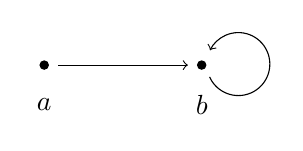
\begin{tikzpicture}
\draw[fill] (0,0) circle (1.5pt);
\draw[fill] (2,0) circle (1.5pt);
\draw[->,shorten >= 5pt, shorten <= 5pt] (0,0) -- (2,0);
\node at (0,-.5) {$a$};
\node at (2,-.5) {$b$};
\draw[->] (2.1,-.15) arc (204:204+310:4mm);
\end{tikzpicture}
\end{center}
De atomaire formule $R(a,b)$ is waar in een situatie als de met $a$ en $b$ aangeduide objecten in een relatie staan die met $R$ overeenkomt. De (binaire) relatie $R$ is met pijlen weergegeven. In dit geval is $R(a,b)$ waar: er gaat een pijl van $a$ naar $b$. Ook kunnen we kijken of samengestelde formules waar zijn in deze structuur:
\begin{itemize}
    \item $\exists y\;R(a,y)$ is waar, want de keuze van $b$ voor $y$ voldoet.
    \item $\forall x\;R(x,x)$ is onwaar, want $(a,a)$ behoort niet tot de pijlrelatie.
    \item $\exists y\forall x\;R(x,y)$ is waar, want neem voor $y$ eens $b$, dan gaat zowel van $a$ als van $b$ een pijl naar $b$.
\end{itemize}
\end{example}
Er is een verschil tussen de objecten $a$ en $b$ in de figuur, waarvan we kunnen \textit{zien} dat ze verschillen, en de constanten $a$ en $b$ in de logische taal, die best hetzelfde object zouden kunnen aanduiden. De constanten in de taal zijn de \textit{namen} die we aan de objecten toekennen. (Net zoals in de propositielogica propositieletters proposities uitdrukken, en in de predikaatlogica predikaatsymbolen predikaten aangeven.) We hadden best $a$ en $b$ hetzelfde object \textit{kunnen} laten aanduiden. Dit zou net als bij pseudoniemen zijn: `Paul Haenen', `Margreet Dolman' en `Dominee Gremdaat' zijn namen voor dezelfde persoon. In de logica zijn constanten namen voor objecten, en hetzelfde object kan met verschillende namen worden aangeduid.

Met connectieven kan nog steeds gerekend worden zoals in de propositielogica. Zo is in de situatie van voorbeeld \ref{vb:pred:model} de formule $R(a,b)\wedge R(b,b)$ waar, omdat $R(a,b)$ en $R(b,b)$ beide waar zijn, terwijl $R(a,b)\rightarrow R(b,a)$ onwaar is; er gaat immers wel een pijl van $a$ naar $b$, maar niet eentje van $b$ naar $a$. Vervolgens kunnen we kwantoren en connectieven weer in formules combineren: $\forall y(\exists x\;R(x,y)\rightarrow R(y,y))$ is waar in de situatie van voorbeeld \ref{vb:pred:model}, want als $y=a$, dan is $\exists x\;R(x,y)$ onwaar en dus de implicatie waar, en als $y=b$, dan zijn $\exists x\;R(x,y)$ en $R(y,y)$ beide waar en ook dan is de implicatie waar.

Een situatie als in voorbeeld \ref{vb:pred:model} heet in de logica een \textit{model}. We kunnen deze notie zien als de generalisering van het begrip waardering in de propositielogica\footnote{\textit{Waardering} in propositielogica is de (systematisch) toekenning van waarheidswaarden aan de propositieletters om zodoende te laten zien dat een formule waar danniet onwaar is; zodoende is elke rij van een waarheidstabel dus een waardering, waarvoor de waarheid van de formule waarvoor de tabel gemaakt wordt geanalyseerd.} (en het is net als inde propositielogica gebruikelijk `model' relatief ten opzichte van een formule, of een verzameling formules, te gebruiken: een situatie is \textit{model} van een formule als de formule daarin waar is). Een model bestaat uit een verzameling objecten waarop een aantal relaties en bewerkingen zijn gegeven die overeenkomen met de predikaat en functiesymbolen. Ook moeten we aangeven welk object uit de gegeven verzameling staat voor welke constante. We laten door middel van een aantal voorbeelden zien hoe modellen werken, en geven geen echte definitie.

Een atomaire formule zoals $R(a,b)$ is \textit{waar} in een model $\mathcal M$ als, gegeven de vertaalsleutel voor $a, b$ en $R$, de met $R$ in $\mathcal M$ corresponderende relatie geldt tussen de in $\mathcal M$ met $a$ en $b$ corresponderende objecten (en net zo voor variabele objecten $x$ en $y$). Een formule $\exists x\;\varphi$ is waar als er een object in $\mathcal M$ is zodat $\varphi$ waar is als we de voorkomens van $x$ in $\varphi$ over dat object laten gaan. Een formule $\forall x\;\varphi$ is waar als dat voor alle objecten in $\mathcal M$ zo is. Als een formule $\varphi$ waar is in $\mathcal M$ dan noteren we dit als $\mathcal M \vDash \varphi$ (de formule volgt \emph{semantisch} uit het model.

\begin{example}
De modellen waarin we predikaatlogica interpreteren kunnen heel abstract zijn maar ook tamelijk concreet. Beschouw bijvoorbeeld het model $\mathcal M$ hierna.
\begin{center}
    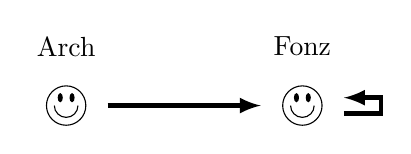
\begin{tikzpicture}
    \draw (0,0) circle (.25cm);
    \draw[fill] (-.075,.1) ellipse (.25mm and .5mm);
    \draw[fill] (.075,.1) ellipse (.25mm and .5mm);
    \draw (-.15,0) arc (180:180+180:1.5mm);
    \node at (0,.75) {Arch};
    \draw (3,0) circle (.25cm);
    \draw[fill] (3-.075,.1) ellipse (.25mm and .5mm);
    \draw[fill] (3+.075,.1) ellipse (.25mm and .5mm);
    \draw (3-.15,0) arc (180:180+180:1.5mm);
    \node at (3,.75) {Fonz};
    \draw[ultra thick,->, shorten <= 15pt, shorten >= 15pt,>=latex] (0,0) -- (3,0);
    \draw[ultra thick, shorten <= 15pt, shorten >= 15pt,->,>=latex] (3, -.1) -- (4, -.1) -- (4, .1) -- (3,.1);
    \end{tikzpicture}
\end{center}
Dit is eigenlijk hetzelfde model als in voorbeeld \ref{vb:pred:model}. Alleen is het linkerobject hier Arch en het rechterobject hier Fonz. Maar Arch en Fonz hadden we net zo goed $a$ en $b$ kunnen noemen. De binaire relatie $R(x,y)$ staat nu voor `persoon $x$ kent persoon $y$'. De drie andere formules in voorbeeld \ref{vb:pred:model} kunnen we nu ook een concretere interpretatie geven:
\begin{itemize}
    \item $\mathcal M \vDash \exists y\;R(a,y)$: `Arch kent iemand'. Dit is waar, want Arch kent Fonz.
    \item $\mathcal M \not\vDash \forall x\;R(x,x)$: `Iedereen kent zichzelf'. Dit is onwaar, want Arch kent zichzelf niet, alleen Fonz kent zichzelf.
    \item $\mathcal M \vDash \exists y\forall x\;R(x,y)$: `Er is iemand die door iedereen gekend wordt'. Dit is waar, want het gaat op voor Fonz.
\end{itemize}
\end{example}

Wanneer er ook nog sprake is van een eenplaatsig predikaatsymbool $P$ (een \textit{eigenschap}), dan geven we behalve pijlen ook gebieden in het model aan (waarin de objecten liggen die de eigenschap hebben) of we markeren de punten die aan een bepaalde eigenschap voldoen afzonderlijk.

\begin{example}\label{vb:pred:model:prop}
We gaan van een aantal formules na of ze waar of onwaar zijn in het model $\mathcal M$ hierna. Dit $\mathcal M$ verbeeldt twee objecten, een eigenschap en een relatie. Object $a$ heeft de eigenschap $P$, wat we aangeven met een open rondje, en de relatie $\{(a,a), (a,b)\}$ komt met $R$ overeen.

\begin{center}
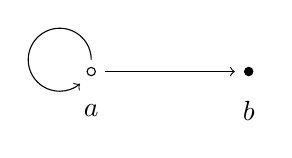
\begin{tikzpicture}
\draw (0,0) circle (1.5pt);
\draw[fill] (2,0) circle (1.5pt);
\draw[->,shorten >= 5pt, shorten <= 5pt] (0,0) -- (2,0);
\node at (0,-.5) {$a$};
\node at (2,-.5) {$b$};
\draw[->] (0,.15) arc (0:0+310:4mm);
\end{tikzpicture}
\end{center}
\begin{itemize}
    \item $\mathcal M \vDash \exists x(P(x)\wedge R(x,x))$\\
    Dit is waar. Ken aan $x$ $a$ toe, dan zien we dat $P(a)$ geldt (object $a$ heeft de eigenschap $P$) en dat $(a,a)\in R$ (de relatie $R$ bestaat tussen $a$ en zichzelf).
    \item $\mathcal M \not\vDash \forall x\exists y\;R(x,y)$\\
    Dit is onwaar. Ken aan $x$ $b$ toe. Er is geen uitgaande pijl van $b$ (er is geen pijl van $b$ naar $b$, en er is ook geen pijl van $b$ naar $a$). Kennelijk is $\exists y\;R(x,y)$ onwaar als $x$ gelijk aan $b$ is. Het geldt dus niet voor alle $x$ dat $\exists y\;R(x,y)$ waar is. Dus $\forall x\exists y\;R(x,y)$ is onwaar.
    \item $\mathcal M \vDash \forall x(P(x)\rightarrow\exists y\;R(x,y))$\\
    Dit is waar. We moeten iets aantonen voor alle $x$. Aan $x$ kunnen we $a$ toekennen, maar ook $b$. In het eerste geval heeft het object de eigenschap $P$, en moeten we laten zien dat er een $y$ is zodat $R(x,y)$. En die is er: ken $b$ aan $y$ toe. In het tweede geval geldt de implicatie omdat het object de eigenschap $P$ niet heeft: $P(b)$ is immers onwaar.
    \item $\mathcal M \vDash \forall x(R(x,x)\rightarrow(P(x)\wedge \exists y(R(x,y)\wedge\neg P(y))))$\\
    Dit is eveneens waar. Je kan zelf de verificatie uitvoeren.
\end{itemize}
Het grappige is dat in deze vier formules $a$ en $b$ nergens genoemd worden, maar dat we er \textit{toch} betekenis aan kunnen geven. Dit zien we vaak in de predikaatlogica.
\end{example}

\begin{example}
Ook in het geval van voorbeeld \ref{vb:pred:model:prop} kunnen we een iets beeldender interpretatie kiezen. Kijk maar eens naar de figuur hierna, die verbeeldt dat: Arch heeft haar, Arch kent zichzelf, en Arch kent Fonz.
\begin{center}
    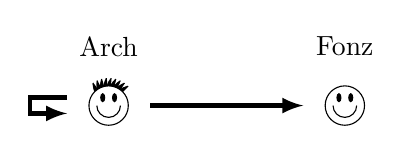
\begin{tikzpicture}
    \draw (0,0) circle (.25cm);
    \draw[fill] (-.075,.1) ellipse (.25mm and .5mm);
    \draw[fill] (.075,.1) ellipse (.25mm and .5mm);
    \draw (-.15,0) arc (180:180+180:1.5mm);
    \node at (0,.75) {Arch};
    \foreach \x in {45,55,...,134} \draw (\x:0.25cm) -- (\x:0.35cm);
    \foreach \x in {46,56,...,134} \draw (\x:0.25cm) -- (\x:0.34cm);
    \foreach \x in {47,57,...,134} \draw (\x:0.25cm) -- (\x:0.33cm);
    \foreach \x in {48,58,...,134} \draw (\x:0.25cm) -- (\x:0.32cm);
    \foreach \x in {49,59,...,134} \draw (\x:0.25cm) -- (\x:0.31cm);
    \foreach \x in {50,60,...,134} \draw (\x:0.25cm) -- (\x:0.30cm);
    \foreach \x in {51,61,...,134} \draw (\x:0.25cm) -- (\x:0.29cm);
    \foreach \x in {52,62,...,134} \draw (\x:0.25cm) -- (\x:0.28cm);
    \foreach \x in {53,63,...,134} \draw (\x:0.25cm) -- (\x:0.27cm);
    \foreach \x in {54,64,...,134} \draw (\x:0.25cm) -- (\x:0.26cm);
    \draw (3,0) circle (.25cm);
    \draw[fill] (3-.075,.1) ellipse (.25mm and .5mm);
    \draw[fill] (3+.075,.1) ellipse (.25mm and .5mm);
    \draw (3-.15,0) arc (180:180+180:1.5mm);
    \node at (3,.75) {Fonz};
    \draw[ultra thick,->, shorten <= 15pt, shorten >= 15pt,>=latex] (0,0) -- (3,0);
    \draw[ultra thick, shorten <= 15pt, shorten >= 15pt,->,>=latex] (0, .1) -- (-1, .1) -- (-1, -.1) -- (0,-.1);
    \end{tikzpicture}
\end{center}
De formules van voorbeeld \ref{vb:pred:model:prop} zijn hier natuurlijk eveneens waar/onwaar. Voor de interpretatie kunnen we bedenken (voor `object' nemen we nu gemakshalve `man'):
\begin{itemize}
    \item $\mathcal M \vDash \exists x(P(x)\wedge R(x,x))$\\
    ``Er is een behaarde man die zichzelf kent.'' Dit is waar: Arch.
    \item $\mathcal M \not\vDash \forall x\exists y\;R(x,y)$\\
    ``Iedereen kent iemand.'' Dit is onwaar. Fonz kent niemand.
    \item $\mathcal M \vDash \forall x(P(x)\rightarrow\exists y\;R(x,y))$\\
    ``Iedere behaarde man kent iemand.'' Dit is ook waar. Arch heeft haar en kent Fonz.
    \item $\mathcal M \vDash \forall(R(x,x)\rightarrow(P(x)\wedge\exists y(R(x,y)\wedge\neg P(y))))$\\
    ``Iedereen met zelfkennis is behaard en kent een kale.''
\end{itemize}
\end{example}

Tot nu gaven we een model $\mathcal M$ en bekeken dan welke formules waar waren. Soms zijn we meer in een andere vraag ge\"interesseerd: gegeven een formule, verzin een model $\mathcal M$ dat deze formule waar (of juist onwaar) maakt. Als dit lukt noemen we de formule vervulbaar\footnote{Merk op dat, terwijl het vinden van een model de vervulbaarheid van een formule aantoont, het vinden van een model dat een formule onwaar maakt, niet de \textit{onvervulbaarheid} van die formule aantoont!}. Dit gaat dus net als in de propositielogica: een formule is vervulbaar als ze een model heeft.

\begin{example}
De formule $\forall x\exists y\;R(x,y)$ is waar in het model van voorbeeld \ref{vb:pred:model} en onwaar in het model van voorbeeld \ref{vb:pred:model:prop}. Voor formule $\forall x\forall y(R(x,y)\rightarrow R(x,x))$ is het omgekeerde het geval: deze is onwaar in het model van voorbeeld \ref{vb:pred:model} en waar in het model van voorbeeld \ref{vb:pred:model:prop}. Ze is onwaar in het eerste model, want neem namelijk $x=a$ en $y=b$, dan is $R(a,b)\rightarrow R(a,a)$ onwaar.

Maar ze is waar in het laatste model, want neem namelijk $x=a$ dan zijn $R(a,a)\rightarrow R(a,a)$ en $R(a,b)\rightarrow R(a,a)$ beide waar en voor $x=b$ zijn ook $R(b,a)\rightarrow R(b,b)$ en $R(b,b)\rightarrow R(b,b)$ beide waar. Beide formules zijn dus vervulbaar.
\end{example}

Tot nu toe hebben we het alleen over modellen voor gesloten formules gehad. Wat te doen met vrije variabelen? Anders dan voor een constante, ligt de waarde van een (vrije) variabele niet vast door het model. Om te kunnen vaststellen of de formule in zo'n geval waar is, moeten de waarden van de vrije variabelen expliciet worden aangegeven. Zo is $P(x)\wedge\exists y\;R(x,y)$ waar in het model van voorbeeld \ref{vb:pred:model:prop} als $x=a$, maar onwaar als $x=b$.
\begin{example}
Beschouw het volgende model. Het bestaat uit de getallen 2, 3, 4 en 5 met de `kleiner dan'-relatie en de priemgetaleigenschap.
\begin{center}
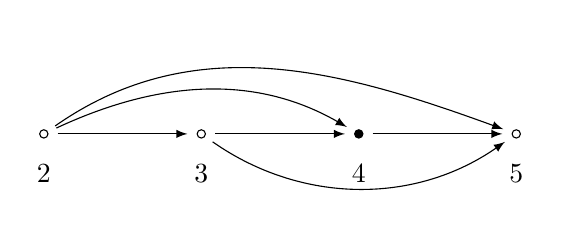
\begin{tikzpicture}
\draw (0,0) circle (1.5pt);
\draw (2,0) circle (1.5pt);
\draw[fill] (4,0) circle (1.5pt);
\draw (6,0) circle (1.5pt);
\draw[->,shorten >= 5pt, shorten <= 5pt,>=latex] (0,0) -- (2,0);
\draw[->,shorten >= 5pt, shorten <= 5pt,>=latex] (2,0) -- (4,0);
\draw[->,shorten >= 5pt, shorten <= 5pt,>=latex] (4,0) -- (6,0);
\node at (0,-.5) {$2$};
\node at (2,-.5) {$3$};
\node at (4,-.5) {$4$};
\node at (6,-.5) {$5$};
\draw[->,shorten <= 5pt, shorten >= 5pt,out=25,in=150,>=latex] (0,0) to (4,0);
\draw[->,shorten <= 5pt, shorten >= 5pt,out=35,in=160,>=latex] (0,0) to (6,0);
\draw[->,shorten <= 5pt, shorten >= 5pt,out=325,in=215,>=latex] (2,0) to (6,0);
\end{tikzpicture}
\end{center}
De constanten 2, 3, 4 en 5 zijn gewoon door die getallen weergegeven. De eigenschap $P$ staat voor `priemgetal' (en is weergegeven door een open rondje). Neem nu de formule $x<5\rightarrow P(x)$. Deze is waar als $x=3$, omdat $3<5$ en 3 een priemgetal is. De formule is daarentegen onwaar als $x=4$, omdat $4<5$ maar 4 is geen priemgetal is. Maar als $x=5$ is de formule waar: 5 is immers \textit{niet} (echt) kleiner dan 5. Voor de waarheid van de implicatie maakt het verder niet uit dat 5 een priemgetal is.
\end{example}

\begin{example}
Hoewel de nadruk tot zover heeft gelegen op eindige modellen, zijn ook oneindige modellen mogelijk. De verzameling van natuurlijke getallen $\mathbb{N}=\{0, 1, 2, 3, 4, \ldots\}$ is het schoolvoorbeeld van een oneindige verzameling. Vat in dit model het predikaatsymbool $P$ op als de verzameling priemgetallen $\{2,3,5,7,11,\ldots\}$, het predikaatsymbool $E$ als de verzameling even natuurlijke getallen $\{0,2,4,6,8,\ldots\}$, en de tweeplaatsige predikaatsymbolen $>$ en $\leq$ als de groter-dan-relatie respectievelijk kleiner-dan-of-gelijk-relatie. Op dit model zijn bijvoorbeeld de volgende formules waar:
$$\forall x(E(x)\rightarrow\exists y((y>x)\wedge E(y)))$$
$$\forall x(P(x)\rightarrow\exists y((y>x)\wedge P(y)))$$
Onwaar zijn:
$$\forall x(E(x)\vee P(x))$$
$$\forall x(P(x)\rightarrow P(x+2))$$
Het functiesymbool `$+$'wordt hier opgevat als gewone optelling. Ten slotte zijn er nog formules waarvan de waarheid onbekend is, zoals het vermoeden van Goldbach:
$$\forall x((E(x)\wedge x>2)\rightarrow\exists y\exists z(P(y)\wedge P(z)\wedge x=y+z))$$
Zoals eerder gezegd staan we in de predikaatlogische taal ook uitdrukkingen als $x+y$ toe als term.
\end{example}

\section{Predikaatlogische wetten en logisch gevolg}
 Net als voor de propositielogica kunnen we ook voor de predikaatlogica \textit{logisch gevolg} en \textit{logische equivalentie} defini\"eren -- met letterlijk dezelfde formuleringen als in hoofdstuk \ref{ch:proposities}. We kunnen dan laten zien dat, bijvoorbeeld, alle vier de volgende formuleringen precies hetzelfde uitdrukken, namelijk dat er geen grootste priemgetal is (zie het voorbeeld aan het begin van sectie \ref{sec:pred:semantiek}):
 \begin{itemize}
     \item $\forall x(P(x)\rightarrow\exists y(P(y)\wedge y>x))$
     \item $\forall x\exists y(P(x)\rightarrow(P(y)\wedge y>x))$
     \item $\forall x\exists y(\neg P(x)\vee(P(y)\wedge y>x))$
     \item $\forall x\exists y((P(x)\rightarrow P(y))\wedge((P(x)\rightarrow y>x))$
 \end{itemize}
 Een voorbeeld van een algemene predikaatlogische wet, die we informeel inmiddels al wel toegepast hebben, is dat $\neg\exists x\;\varphi$ equivalent is met $\forall x\;\neg\varphi$. Met zo'n regel, en nog een variatie erop, kunnen we aantonen dat $\forall x\exists y\;x<y$, voor `er is geen grootste getal', logisch equivalent is met de formule $\neg\exists x\forall y\;x\geq y$ - we gebruiken daarin tevens dat $\neg(x<y)$ equivalent is met $x\geq y$.
 
 Met de notie van \textit{predikaatlogisch gevolg} kunnen we formeel laten zien dat een eeuwenoude redenering inderdaad geldig is:
 $$\forall x(M(x)\rightarrow S(x)), M(s)\Rightarrow S(s)$$
 Deze formule formaliseert de redenering `Alle mensen zijn sterfelijk. Socrates is een mens. Dus Socrates is sterfelijk.'
 
 Een volgend voorbeeld van een standaard predikaatlogisch gevolg  is $\exists x\forall y\;\varphi\Rightarrow\forall y\exists x\;\varphi$\footnote{Maak zelf een model om dit te verifi\"eren.}. Maar in de andere richting is dit nu juist ongeldig: neem bijvoorbeeld voor $\varphi$ de atomaire formule $y>x$ en als model de natuurlijke getallen, dan is $\forall y\exists x\;x>y$ het geval want bij ieder natuurlijk getal is er nog een groter natuurlijk getal, bijvoorbeeld dat getal plus 1. Maar $\exists x\forall y\;x>y$ is onwaar, want er is geen grootste natuurlijk getal. Dus $\forall y\exists x\;x>y\not\Rightarrow\exists x\forall y\;x>y$.
 
 \section{Samenvatting}
 Voor het bepalen van de waarheidswaarde van een formule spelen in de predikaatlogica modellen dezelfde rol als waarderingen in de propositielogica. Een model is een structuur die bestaat uit een verzameling objecten waarop relaties (en in het bijzonder: eigenschappen) zijn gedefinieerd. De relaties komen overeen met de predikaatsymbolen van de formules waaraan we een waarheidswaarde willen toekennen. Objecten kennen we aan de constanten in de predikaatlogische taal toe. Verschillende constanten kunnen in een model hetzelfde object aanduiden, en een constante kan in verschillende modellen door verschillende objecten worden weergegeven. Voor variabelen kunnen we in een gegeven model verschillende waarden kiezen. Een formule $\forall x\;\varphi$ is waar als $\varphi$ geldt voor elk object dat we aan $x$ kunnen toekennen; $\exists x\;\varphi$ is waar als er ten minste \'e\'en zo'n object bestaat.
 
 \subsection{Opgaven}
 \begin{exercise}
 Stel we gebruiken het functiesymbool `$-$' voor de bewerking `aftrekken'. Als $E$ staat voor `is even' en `$P$' voor `is een priemgetal', wat drukken de volgende formules dan uit?
 \begin{enumerate}
     \item $\forall x((E(x)\wedge x>2)\rightarrow\exists y(P(y)\wedge P(x-y)))$
     \item $\neg\exists x(P(x)\wedge\forall y(P(y)\rightarrow y\leq x))$
 \end{enumerate}
 \end{exercise}
 
 \begin{exercise}
 Beschouw de formule $\forall x\forall y\forall z((R(x,y)\wedge R(y,z))\rightarrow R(x,z))$.
 \begin{enumerate}
     \item Is deze formule waar in een model $\mathcal M$ met de natuurlijke getallen als objecten, waarin $R$ overeenkomt met de gewone kleiner-dan-relatie ($<$)?
     \item En in een model $\mathcal N$ met dezelfde verzameling objecten, maar nu met de relatie $R$ gedefinieerd door: $R(x, y)$ precies dan als $x\leq y+1$?
     \item Is de formule waar in het model $\mathcal O$ uit voorbeeld \ref{vb:pred:model}?
     \item Is de formule waar in elk model $\mathcal P$ met precies twee objecten? Zo ja, bewijs dit, zo nee, geef een voorbeeld van een model met twee objecten waarop de formule niet waar is.
 \end{enumerate}
 \end{exercise}
 
\begin{exercise}
Beschouw het volgende model $\mathcal M$:
\begin{center}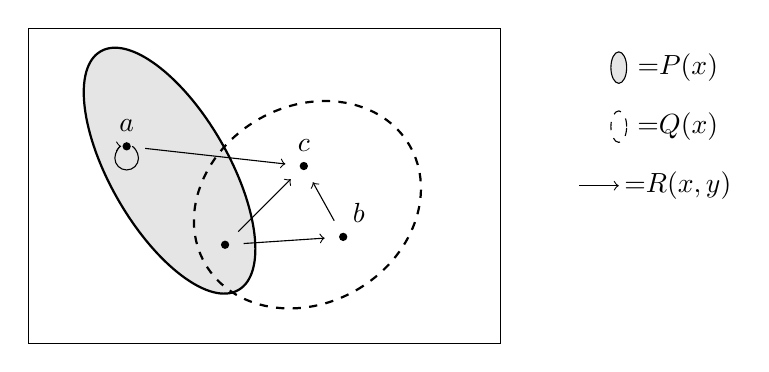
\begin{tikzpicture}
\draw (0,0) rectangle (6,4);
\draw[thick,fill=gray!20,rotate=30] (2.65,1) ellipse (.75cm and 1.75cm);
\draw[thick,dashed,rotate=-60] (.25,3.95) ellipse (1.25cm and 1.5cm);
\node[circle,fill,inner sep=0pt,minimum size=3pt,label={[anchor=south]north:$a$}] at (1.25, 2.5) (a) {};
\node[circle,fill,inner sep=0pt,minimum size=3pt] at (2.5, 1.25) (d) {};
\node[circle,fill,inner sep=0pt,minimum size=3pt,label={[anchor=south west]north:$b$}] at (4,1.35) (b) {};
\node[circle,fill,inner sep=0pt,minimum size=3pt,label={[anchor=south]north:$c$}] at (3.5,2.25) (c) {};
\draw[->,shorten <=2pt,shorten >=2pt] (a) arc(90:-270:.15); 
\draw[->,shorten <=5pt,shorten >=5pt] (a) -- (c); 
\draw[->,shorten <=5pt,shorten >=5pt] (d) -- (c); 
\draw[->,shorten <=5pt,shorten >=5pt] (d) -- (b); 
\draw[->,shorten <=5pt,shorten >=5pt] (b) -- (c);
\draw[fill=gray!20] (7.5,3.5) ellipse (.1cm and .2cm);\node at (8.25,3.5) {=$P(x)$};
\draw[dashed] (7.5,2.75) ellipse (.1cm and .2cm);\node at (8.25,2.75) {=$Q(x)$};
\draw[->] (7,2) -- (7.5,2);\node at (8.25,2) {=$R(x,y)$};
\end{tikzpicture}
\end{center}
Beredeneer welke van de volgende formules geldig zijn op $\mathcal M$:
\begin{enumerate}
    \item $\mathcal M \vDash R(a,a)$
    \item $\mathcal M \vDash R(x,x)$
    \item $\mathcal M \vDash \exists y\; R(a,y)$
    \item $\mathcal M \vDash \exists x\; R(x,x)$
    \item $\mathcal M \vDash \neg\forall x(P(x)\rightarrow R(x,x))$
    \item $\mathcal M \vDash \exists x(P(x)\wedge R(x,x))$
    \item $\mathcal M \vDash \forall x\exists y\;R(x,y)$
    \item $\mathcal M \vDash \forall x(R(x,x)\rightarrow P(x))$
    \item $\mathcal M \vDash \forall x\bigl[P(x)\rightarrow\exists y\;R(x,y)\bigr]$
    \item $\mathcal M \vDash \forall x\bigl[P(x)\rightarrow\exists y(R(x,y)\wedge Q(y))]$
\end{enumerate}
\end{exercise}

\begin{exercise}
Beschouw het domein $\mathbb{N}$ van natuurlijke getallen, met $E$ als het even-predikaat ($E(x)$ wil zeggen `$x$ is even') en een $A$ als optel-predikaat ($A(x,y,z)$ wil zeggen `$x+y=z$').

Geef aan of de volgende zinnen waar zijn op dit model:
\begin{enumerate}[label=\textit{\alph*.}]
\item $\forall x(E(x)\leftrightarrow\exists y\;A(y,y,x))$;
\item $\forall z\exists x\exists y(\neg(x=y)\wedge A(x,y,z))$;
\item $\forall x\forall y\forall z((E(x)\wedge E(y)\wedge A(x, y, z))\rightarrow E(z))$.
\end{enumerate}
\end{exercise}

\begin{exercise}
Gegeven is de volgende informatie over een model:\\
Predikaten $P,Q$ en $P$ is een-plaatsig, $Q$ is twee-plaatsig.\\
1 constante $c$.
$$A:= \forall x (P(x)\rightarrow\exists y\; Q(x,y))$$
\begin{enumerate}[label=\textit{\alph*.}]
\item Teken een model $\mathcal M$ waar deze formule waar is.
\item Teken een model $\mathcal N$ waar deze formule onwaar is.
\end{enumerate}
$$B:=(P(c)\wedge\forall x(P(x)\rightarrow\exists y(Q(x,y)\wedge P(y))))$$
\begin{enumerate}[label=\textit{\alph*.}]
\setcounter{enumi}{2}
\item Hoeveel elementen heb je minimaal nodig in een model om $B$ waar te maken?
\end{enumerate}
\end{exercise}
